\section{Aplicación de RK4}\label{sect:application}

Ya se introdujo a los métodos numéricos de Runge-Kutta y se describió el más popular, RK4. A continuación, para seguir con el desarrollo de este método, se describirá una aplicación en la cual este método puede ser aplicado.

\subsection{Oscilador de Van der Pol}

Recordemos que un oscilador es un sistema dinámico que presenta una especie de variación estable y periódica a lo largo del tiempo. Uno de los osciladores más sencillos es el oscilador armónico amortiguado, que es descrito por la siguiente ecuación diferencial ordinaria de segundo orden:
\[
	\frac{d^2 y}{dx^2} + \mu \frac{dy}{dx} + y = 0
\]
Aquí, \(\mu\) es un parámetro escalar que controla el amortiguamiento del sistema (sobreamortiguamiento, amortiguamiento crítico o subamortiguamiento). Las soluciones a esta ecuación diferencial pueden ser obtenidas analíticamente de forma relativamente sencilla, así que no nos enfocaremos en esta aplicación.

En lugar, preferiremos como sujeto de estudio al \textbf{oscilador de Van der Pol}. Este tipo de oscilador, nombrado en honor al físico e ingeniero eléctrico neerlandés Balthasar van der Pol, tiene una amortiguación no lineal, lo que resulta en un comportamiento curioso que a lo largo del tiempo es descrito por la siguiente ecuación diferencial ordinaria de segundo orden:
\begin{equation} \label{eq:van-der-pol}
	\frac{d^2 x}{dt^2} - \mu (1 - x^{2}) \frac{dx}{dt} + x = 0
\end{equation}
…donde \(x\) representa la coordenada de la posición (en función de \(t\)) y \(\mu\) es un parámetro escalar que controla la no linearidad y la fuerza del amortiguamiento. Esta ecuación es algunas veces llamada simplemente la «ecuación de Van der Pol».

Esta ecuación tiene muchas aplicaciones, que van desde la física y la electrónica hasta la biología. Originalmente fue utilizada para describir las oscilaciones de un circuito de tubos de vacío, pero más recientemente ha sido utilizada para describir el comportamiento de las neuronas y para el desarrollo de un modelo que describe la interacción entre dos placas geológicas, solo por citar un par de ejemplos.

Debido a que la ecuación de Van der Pol no es lineal, es imposible la obtención de una solución analítica exacta en términos de funciones elementales conocidas. Por ello, el único camino que tenemos para analizar su solución son los métodos numéricos. Utilizaremos el método RK4 para encontrar numéricamente las soluciones a esta ecuación.

\subsection{Van der Pol en Términos de Ecuaciones de Primer Orden}

Antes de poder utilizar el método de Runge-Kutta de grado 4 para la obtención de las soluciones numéricas de la ecuacióned Van der Pol, debemos notar que no podemos aplicarlo de manera directa sobre la ecuación~(\ref{eq:van-der-pol}), pues, recordemos que, tal como fue descrito en la sección~\ref{sect:def-rk4}, el método necesita de una ecuación de \textit{primer} orden de la forma de~(\ref{eq:main-diff-eq}).

No obstante, podemos establecer \(y = \frac{dx}{dt}\), y así podemos reescribir la ecuación~(\ref{eq:van-der-pol}) como un sistema de dos ecuaciones diferenciales ordinarias de primer orden:
\begin{equation} \label{eq:system-van-der-pol}
	\begin{cases}
		\dfrac{dx}{dt} &= y \\[1em]
		\dfrac{dy}{dt} &= \mu(1 - x^{2})y - x
	\end{cases}
\end{equation}
De esta forma, ya tenemos dos ecuaciones de la forma necesaria para utilizar el método RK4.

\subsection{Solución con RK4}

Para encontrar las soluciones al sistema~(\ref{eq:system-van-der-pol}) se tendrá que resolver cada una de las ecuaciones de forma independiente con valores iniciales distintos para \(x\) y \(y\), pero cuidando que el valor inicial y el intervalo de \(t\), así como el tamaño \(h\) de los pasos, sean los mismos para ambas ecuaciones.

Si bien se podría realizar el procedimiento del método RK4 a mano, es más conveniente el desarrollo de un programa que lo realice computacionalmente, ahorrándonos tiempo y esfuerzo. Después de todo, la utilización de los métodos numéricos para la obtención de soluciones a ecuaciones diferenciales ordinarias (y muchas otras aplicaciones) se ha vuelto especialmente viable en las últimas décadas luego de los avances en la velocidad de procesamiento computacional.

El programa fue realizado en Python, un lenguaje de programación popular para este tipo de aplicaciones. La implementación de RK4 en Python es sumamente sencilla y solo se utilizaron los paquetes \textit{numpy} para un manejo más elegante de los cálculos, y \textit{matplotlib} para la graficación de la solución obtenida. El código se encuentra en la sección~\ref{sect:python} y también está disponible en el \href{https://github.com/camargomau/runge-kutta}{repositorio de GitHub de este documento}.

El funcionamiento del programa es simple:
\begin{enumerate}
    \item Se obtienen los datos que el usuario debe definir antes de la aplicación de RK4.
    \item En base a esos datos, se definen las estructuras necesarias para la aplicación de RK4.
    \item Una vez se tienen las estructuras, se procede a la aplicación de RK4, iterando a lo largo del conjunto discreto de \(t\).
    \item Cuando se termina la aplicación del método, se guarda la solución final y luego se representa en dos gráficas: una donde se trazan individualmente \(x\) y \(y\) contra \(t\), y otra donde se traza \(x\) contra \(y\).
\end{enumerate}

\subsubsection{Ejemplo 1}

Ya que tenemos un programa que realiza los cálculos de forma sencilla, podemos experimentar con los parámetros y demás valores que uno define antes de comenzar la aplicación de RK4.

Para un primer ejemplo, utilizaremos:
\begin{align*}
    \mu &= 1 \\
    x_{0} = 1 &\qquad y_{0} = 0 \\
    t_{0} = 0 &\qquad t_{\text{final}} = 50 \\
    h &= 0.01
\end{align*}
Introducimos estos datos al programa:
\begin{figure}[H]
	\centering
	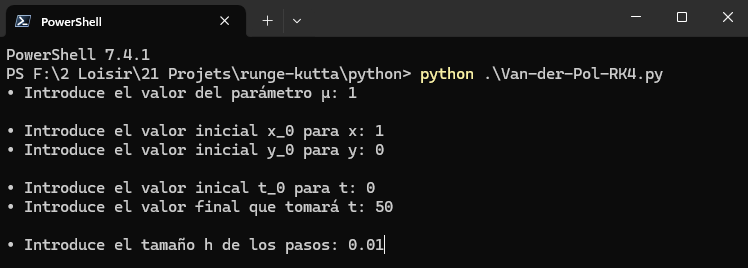
\includegraphics[scale=0.65]{../auxiliary/assets/ejemplo1-datos.png}
	\caption{Introducción de los datos del ejemplo 1 al programa desde PowerShell}
\end{figure}
Posteriormente, el programa aproxima la solución a la ecuación de Van der Pol correspondiente (en su forma de sistema de ecuaciones de primer orden) utilizando el método RK4 con la configuración que hemos definido según estos datos y finalmente nos muestra las gráficas correspondientes a la solución encontrada:
\begin{figure}[H]\label{fig:ej1}
	\centering
	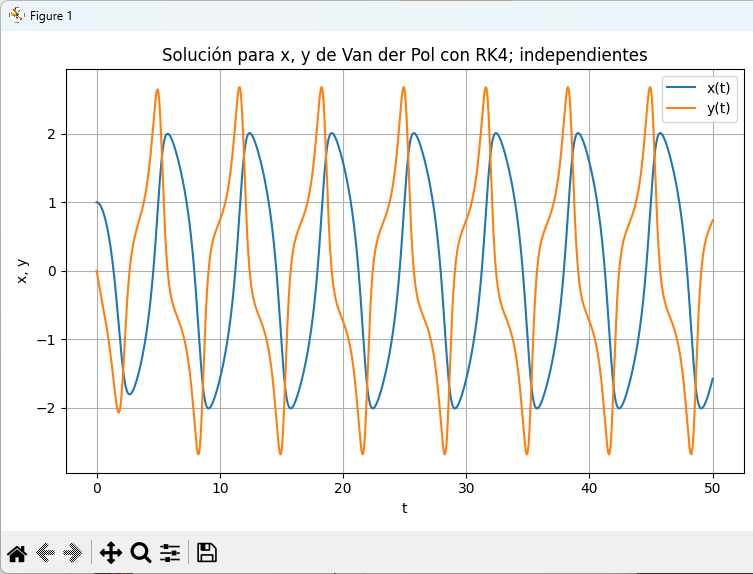
\includegraphics[scale=0.5]{../auxiliary/assets/ejemplo1-indiv.png}
	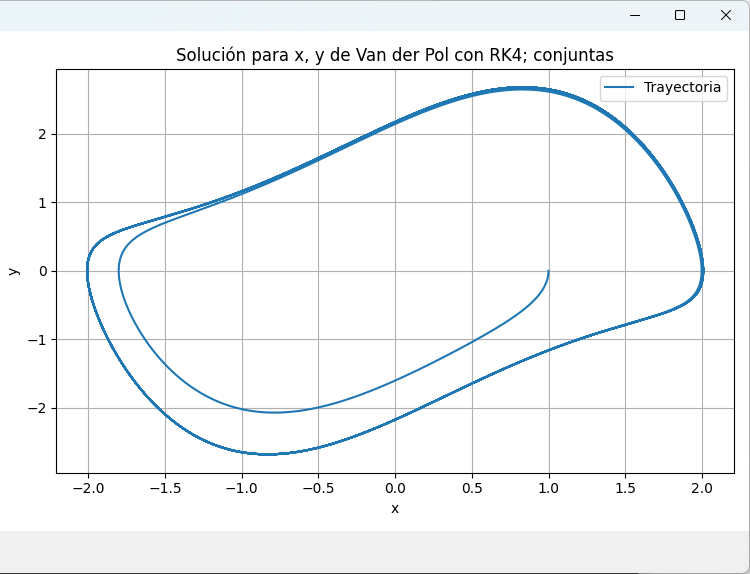
\includegraphics[scale=0.5]{../auxiliary/assets/ejemplo1-conj.png}
	\caption{Gráficas de las soluciones halladas correspondientes al ejemplo 1}
\end{figure}
Si buscamos en diversas fuentes sobre el oscilador de Van der Pol y las soluciones a su ecuación (como las que están en la sección de referencias), comprobaremos que efectivamente toman la forma de las gráficas que hemos obtenido con el programa. El programa funciona correctamente.

Un análisis del comportamiento de las soluciones a la ecuación de Van der Pol en sí está fuera del alcance de este documento, así que enfoquémonos solamente en el análisis del procedimiento numérico. Podemos observar que, efectivamente, se aproximó la solución en el intervalo \(t \in [0, 50]\) con un paso de \(h = 0.01\). El paso es lo suficientemente pequeño como para resultar en una solución que, al menos a primera vista, parece perfectamente suave sin cambios bruscos o «artefactos».

\subsubsection{Ejemplo 2}

Para resaltar la naturaleza numérica de estas soluciones, se reutilizarán todos los datos del ejemplo 1 para obtener otra solución, pero esta vez optando por un tamaño de paso más largo \(h = 0.75\). Con ello, el programa resulta en:
\begin{figure}[H]
	\centering
	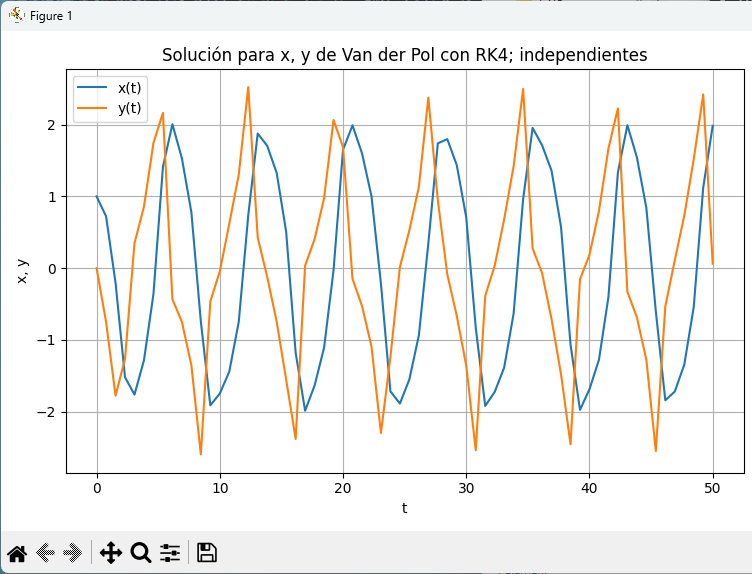
\includegraphics[scale=0.5]{../auxiliary/assets/ejemplo2-indiv.png}
	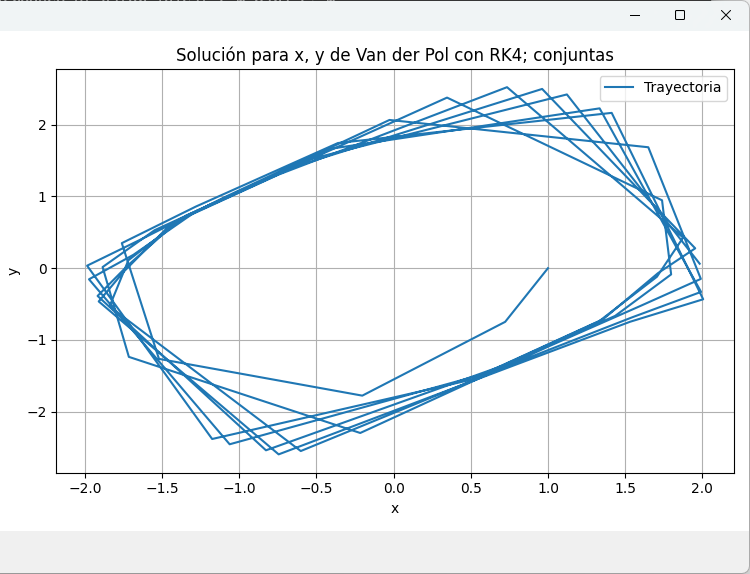
\includegraphics[scale=0.5]{../auxiliary/assets/ejemplo2-conj.png}
	\caption{Aplicación de RK4 con los mismos datos del ejemplo 1, pero \(h = 0.75\)}
\end{figure}
Observemos que esta aproximación continúa teniendo la misma tendencia que la del ejemplo 1 (la solución es la misma, después de todo), pero, esta vez, como el paso es más largo, se perciben los segmentos de recta individuales que unen los puntos de aproximación obtenidos numéricamente.

Aquí también podemos incluso notar de forma más clara que la gráfica conjunta de la aproximación obtenida anteriormente (figura~\ref{fig:ej1}) se compone de una línea que pasa varias veces por puntos muy cercanos; en el ejemplo 1 parecería que es una sola línea que solo pasa una vez por una cierta vecindad, pero en este segundo ejemplo vemos que en realidad pasa varias ocasiones.

\subsubsection{Ejemplo 3}

Como último ejemplo, se mostrará que el programa también funciona para el problema generado por otros datos. Esta vez, se utilizará:
\begin{align*}
    \mu &= 4 \\
    x_{0} = 1 &\qquad y_{0} = 2.5 \\
    t_{0} = 10 &\qquad t_{\text{final}} = 30 \\
    h &= 0.05
\end{align*}
La solución aproximada generada por el programa es:
\begin{figure}[H]
	\centering
	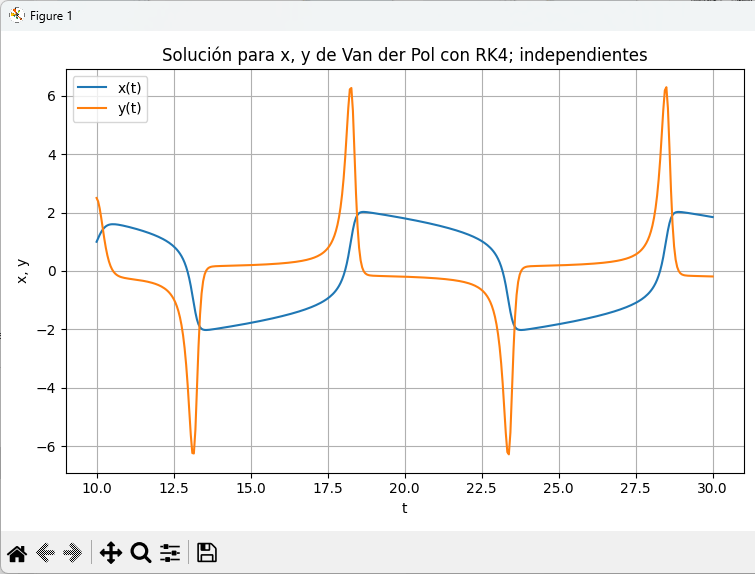
\includegraphics[scale=0.5]{../auxiliary/assets/ejemplo3-indiv.png}
	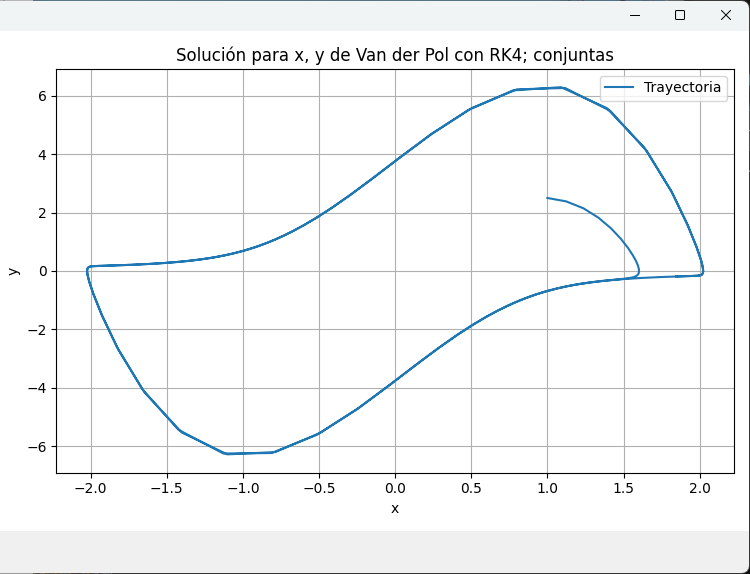
\includegraphics[scale=0.5]{../auxiliary/assets/ejemplo3-conj.png}
	\caption{Aplicación de RK4 con los datos correspondientes al ejemplo 3}
\end{figure}
Notemos que el programa una vez más logra dar una solución aproximada satisfactoria que corresponde al comportamiento de la solución a la ecuación de Van der Pol.
